\subsection{Pilot-selected targets and a matched prior-sensitivity comparison}
To avoid evaluating only a central feature that may miss the pilot's strongest
density, a development protocol locks three regions per stack using only the
old independent pilot. Candidate centers are the $24^3$ cell centers inside
radius $0.30$ of the field. Greedy descending positive pilot scores, with
lexicographic ties and $40\,\AA$ minimum separation, select three Gaussian
averages of standard deviation $20\,\AA$. A matched-width central average is
retained as a fourth target. All twelve target definitions and pilot hashes
are locked before evaluating these feature outcomes. The reference volumes
have been examined elsewhere in development; this is not a new confirmation.
The sampled radius-12 band endpoints are $40.2$, $19.68$, and $34.93\,\AA$,
so the target sigma is not a claim of $20\,\AA$ reconstruction resolution.

The matched Fourier baseline uses the same 128 particles, geometry seed,
prescribed white-noise scale, pilot, reference generator, and target definitions
as this feature study. We evaluate the full and diagonal posteriors on the
same $33^3$ Hermitian grid as above, retaining prior RMS deviation norms
$s=0.5,1,2$, or coordinate SD $s/\sqrt{33^3}$. Each marginal credible interval
uses $\alpha=0.05/12$ for a family of twelve targets at a fixed prior scale.
The variance identity agrees to $2.4\times10^{-13}$ relative error, and the
full matched prior-predictive coverage is $0.995833$ throughout.
Pointwise coverage for a fixed density answers a different question.

After the original three-prior outcomes showed poor pointwise coverage at
several targets, we declared a separate sensitivity using coordinate SDs
$0.1$ and $1$, retaining both on all targets. Their RMS deviation norms are
approximately $19.0$ and $189.6$, much broader than a hard radius-two class.
The original outcomes remain unchanged; these extra priors are post-outcome
development, not a selected replacement. Broadening the prior substantially
improves many nominal-reference results (Table~\ref{tab:pilot-fourier} and
Figure~\ref{fig:pilot-fourier}). At coordinate SD one, nominal full-posterior
coverage ranges from $0.9872$ to $0.9998$, with relative half-widths
$0.016$--$0.074$. This is a material favorable baseline result.
Finite interpolation discrepancy is still $16.8\%$, $16.3\%$, and $25.1\%$
on the respective continuous generators. Matched-model and continuous-signal
checks are retained separately, including the prescribed pose perturbations.
Diagonal VI is wider on every tested target, by factors $1.003$--$1.732$
across all five priors. These checks neither refute Bayesian calibration nor
validate any of the intervals for unknown experimental density.

\begin{table*}[t]
\centering\small
\begin{tabular}{lrrr}
\toprule
Stack & Prior RMS norm & Relative half-width & Pointwise coverage\\
\midrule
10028 & 0.5 & 0.004--0.004 & 0.000--0.000\\
10028 & 1 & 0.006--0.006 & 0.000--0.727\\
10028 & 2 & 0.009--0.009 & 0.003--0.998\\
10028 & 19.0* & 0.012--0.012 & 0.990--0.997\\
10028 & 189.6* & 0.016--0.017 & 1.000--1.000\\
10049 & 0.5 & 0.004--0.004 & 0.000--0.000\\
10049 & 1 & 0.007--0.007 & 0.000--0.000\\
10049 & 2 & 0.014--0.014 & 0.000--0.574\\
10049 & 19.0* & 0.046--0.053 & 0.997--0.999\\
10049 & 189.6* & 0.062--0.074 & 0.987--0.996\\
10076 & 0.5 & 0.004--0.004 & 0.000--0.000\\
10076 & 1 & 0.007--0.007 & 0.000--0.000\\
10076 & 2 & 0.013--0.014 & 0.000--0.000\\
10076 & 19.0* & 0.033--0.034 & 0.964--0.981\\
10076 & 189.6* & 0.036--0.037 & 0.990--0.993\\
\bottomrule
\end{tabular}
\caption{Full Fourier-posterior ranges over all four locked targets per stack at nominal poses. Widths use the continuous radius-two no-data scale only for display; the priors are not hard balls. Every prior is retained. Asterisks denote the broader-prior sensitivity specified after the original baseline outcomes. Pointwise coverage integrates prescribed white Gaussian measurement noise for the fixed continuous map generator; it is not experimental-density calibration.}
\label{tab:pilot-fourier}
\end{table*}

\begin{figure*}[t]
\centering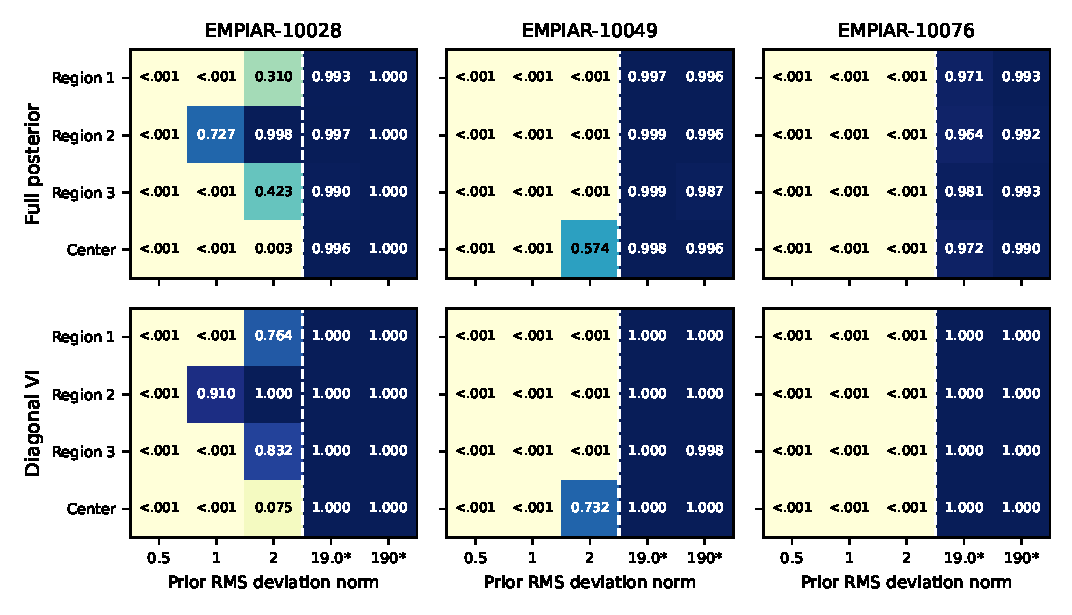
\includegraphics[width=\textwidth]{figures/pilot-selected-fourier.pdf}
\caption{Analytic known-noise pointwise coverage at nominal poses for the four
locked targets per stack. Values are rounded; $1.000$ need not equal one.
The first three columns are the original prior sweep; starred columns are
the separately declared broader-prior sensitivity after those outcomes.
Full matched prior-predictive coverage is $0.995833$ for every prior, whereas
these fixed-reference probabilities need not match it. The improving broader
priors and wider diagonal intervals are retained without selecting a winner.}
\label{fig:pilot-fourier}
\end{figure*}

The broader-prior advantage also persists under the two specified pose
patterns. At coordinate SD one, full-posterior fixed-generator coverage across
the one- and two-degree coherent/random checks is $0.9861$--$0.9999$;
diagonal VI gives at least $0.9978$. These are favorable baseline results,
although the full posterior does not uniformly attain the nominal marginal
$0.995833$ level. They are checks on particular generators and perturbations,
not a worst-case nuisance guarantee. The minimum full-posterior sign power is
$0.0428$, so high coverage alone still does not imply detection of every target.
All five priors and eight scenarios remain in the descriptive summary of the
original 960 checks; regrouping them adds no independent experiments.

All twelve continuous fixed-pose fits are complete and meet their declared
numerical stopping criterion (Table~\ref{tab:lockedfixed}). Their largest
sum-objective gap is 0.00437; each fit takes 2,033--3,613 seconds on the Mac
under concurrent load. The third EMPIAR-10049 pilot region has sign power
0.0158 even at fixed poses, while the other eleven exceed 0.99999 in the
known-noise reference calculation. This unfavorable feature remains in the
family. The nonlinear pose audits and full conditional experimental comparison
are still running. The reserved calibration cohort uses one particle from each
of 128 previously unused exposures per stack, excluding both existing image
pools. All twelve estimators and 116 input/source files were locked and
published before any reserved pixels were downloaded. All three downloads are
complete and verified; the frozen recalibration awaits the full original
feature application. The old inference images remain development data, and neither a fresh
calibration pool nor approximate-map inclusion establishes the density or pose
bounds.
\begin{table}[t]
\centering
\setlength{\tabcolsep}{4.5pt}
\caption{Completed fixed-pose, known-noise calculations for all twelve locked targets (four per stack). Width is relative to no data; power uses the processed-map generator. These are conditional calculations, not experimental coverage.}
\label{tab:lockedfixed}
\begin{tabular}{lrrr}
\toprule
Stack & Width range & Min. sign power & Max. gap\\
\midrule
10028 & 0.0202--0.0202 & $>0.99999$ & 0.00132\\
10049 & 0.0533--0.0539 & 0.0158 & 0.00437\\
10076 & 0.0347--0.0347 & $>0.99999$ & 0.00112\\
\bottomrule
\end{tabular}
\end{table}

